\documentclass[preview,border=5pt]{standalone}
\usepackage{teaching}
\begin{document}

\centering
\pgfplotsset{compat=newest,width=\textwidth}
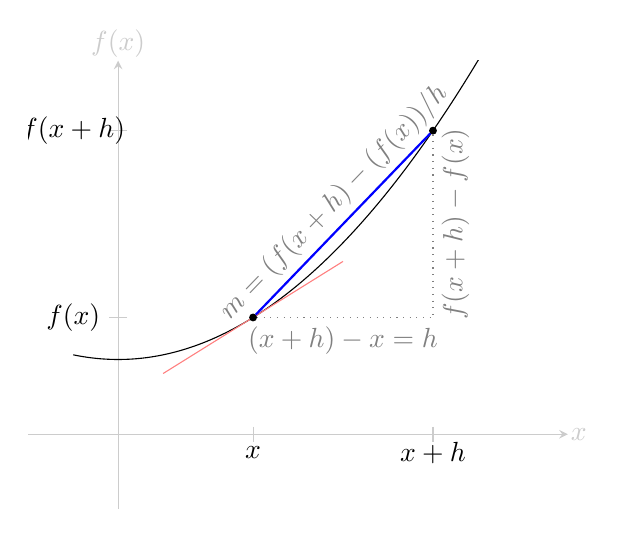
\begin{tikzpicture}[scale=1,inner sep=0.3mm]
\begin{axis}[
axis x line=center,
axis y line=center,
axis line style={black!20!white},
xlabel={$x$},
ylabel={$f(x)$},
xlabel style={right,black!20!white},
ylabel style={above,black!20!white},
samples=128,
ticks=none,
no marks,
xmin=(-1), xmax=(5),
ymin=(-1), ymax=(5)
]
\addplot [black, domain=-0.5:6] {\x^2/4 + 1};
\addplot [red!50!white,domain=0.5:2.5] {3*\x/4 + 0.4375};
\node (a) at (1.5,1.5625) [circle,draw,fill=black] {};
\node (b) at (3.5,4.0625) [circle,draw,fill=black] {};
\draw [thick,blue] (a) -- (b);
\node (c) at (3.5,1.5625) {};
\draw [dotted,black!50!white] (a) -- (c);
\draw [dotted,black!50!white] (b) -- (c);
\node (xhx) at (2.5,1.25) [color=black!50!white] {$(x+h) - x = h$};
\node (fxhfx) at (3.75,2.8125) [color=black!50!white,rotate=90] {$f(x+h) - f(x)$};
\node at (2.4,3.1) [color=black!50!white,rotate=46] {$m = (f(x+h) - (f(x))/h$};
\draw [black!20!white] (1.5,0.1) -- (1.5,-0.1);
\draw [black!20!white] (3.5,0.1) -- (3.5,-0.1);
\node (x) at (1.5,-0.25) {$x$};
\node (xh) at (3.5,-0.25) {$x+h$};
\draw [black!20!white] (0.1,1.5625) -- (-0.1,1.5625);
\draw [black!20!white] (0.1,4.0625) -- (-0.1,4.0625);
\node (fx) at (-0.5,1.5625) {$f(x)$};
\node (fxh) at (-0.5,4.0625) {$f(x+h)$};
\end{axis} 
\end{tikzpicture}

\end{document}